\documentclass[runningheads,a4paper]{article}
\usepackage[utf8]{inputenc}
\setcounter{tocdepth}{3}
\usepackage[english]{babel} 
\usepackage{graphicx}
\usepackage{grffile}
\usepackage{float}
\usepackage{multicol}
\usepackage{url}
\usepackage{titling}
\usepackage[hidelinks]{hyperref}
\setcounter{secnumdepth}{5}
%Margins
\usepackage[
margin=2cm,
includefoot
]{geometry}
\graphicspath{{img/}}
%Headers and Footers
\usepackage{fancyhdr}
\pagestyle{fancy}
\fancyhead{}
\fancyfoot{}
\fancyfoot[R]{\thepage}
\renewcommand{\headrulewidth}{0pt}
\renewcommand{\footrulewidth}{0pt}
\setlength\parindent{24pt}
\begin{document}
%Title Page
\begin{titlepage}
\begin{center}

\includegraphics[width=10cm]{UP.jpg}  \\
[1cm]
\line(1,0){300} \\
[0.3cm]
\textsc{\Large
NavUP \\
Architectural Requirements Specifications and Design \\
\hfill \break 01 March 2017
%University of Pretoria
}\\
[0.1cm]
\line(1,0){300} \\
[0.7cm]
\textsc{\Large
Team MatLab
} \\
\end{center}
\begin{center}
\begin{multicols}{2}
\textsc{\large\\
Frederick Ehlers\\ 
u11061112\\ 
}
\textsc{\large\\
Vignesh Iyer\\
u15031625\\ 
}
\textsc{\large\\
Stephanie Groutsch\\
u14293324\\ 
}
\textsc{\large\\
Neo Thokoa\\
u14163285\\
}
\columnbreak
\textsc{\large\\
Nokuthula Manana\\
u12064115\\
}
\textsc{\large\\
Jacobus Marais\\
u15188397\\
}
\textsc{\large\\
Heinrich Burgers\\
u15059538\\
}
\end{multicols}
\textsc{	\\ \href{https://github.com/FredJEhlers/Matlab}{GitHub}
\url{https://github.com/FredJEhlers/Matlab}}
\end{center}
\end{titlepage}

%\maketitle



\begingroup



\tableofcontents

\addcontentsline{toc}{section}{Table Of Contents}

\endgroup

\newpage




\section{External Interface Requirements}


\section{Performance Requirements}


\section{Design Constraints}


\section{Software System Attributes}


\section{UML Diagrams for the Chosen Subsystems}

Design Patterns have been integrated and a discussion of their use are made below the respective diagrams.


\begin{figure}[H]
   	\centering
   	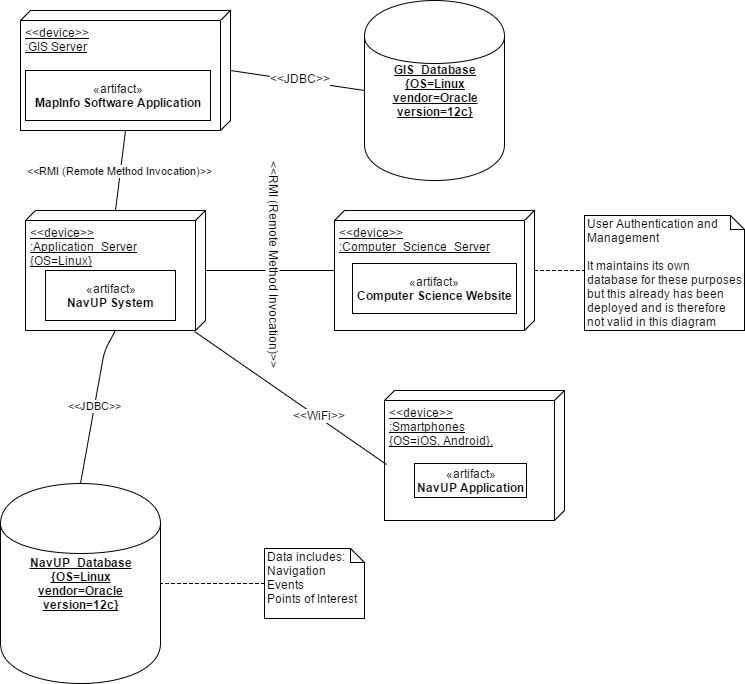
\includegraphics[width=0.7\textwidth]{DeploymentDiagram.jpg}
   	\caption{Deployment Diagram for NavUP}
\end{figure}


\subsection {User}

\begin{figure}[H]
   	\centering
   	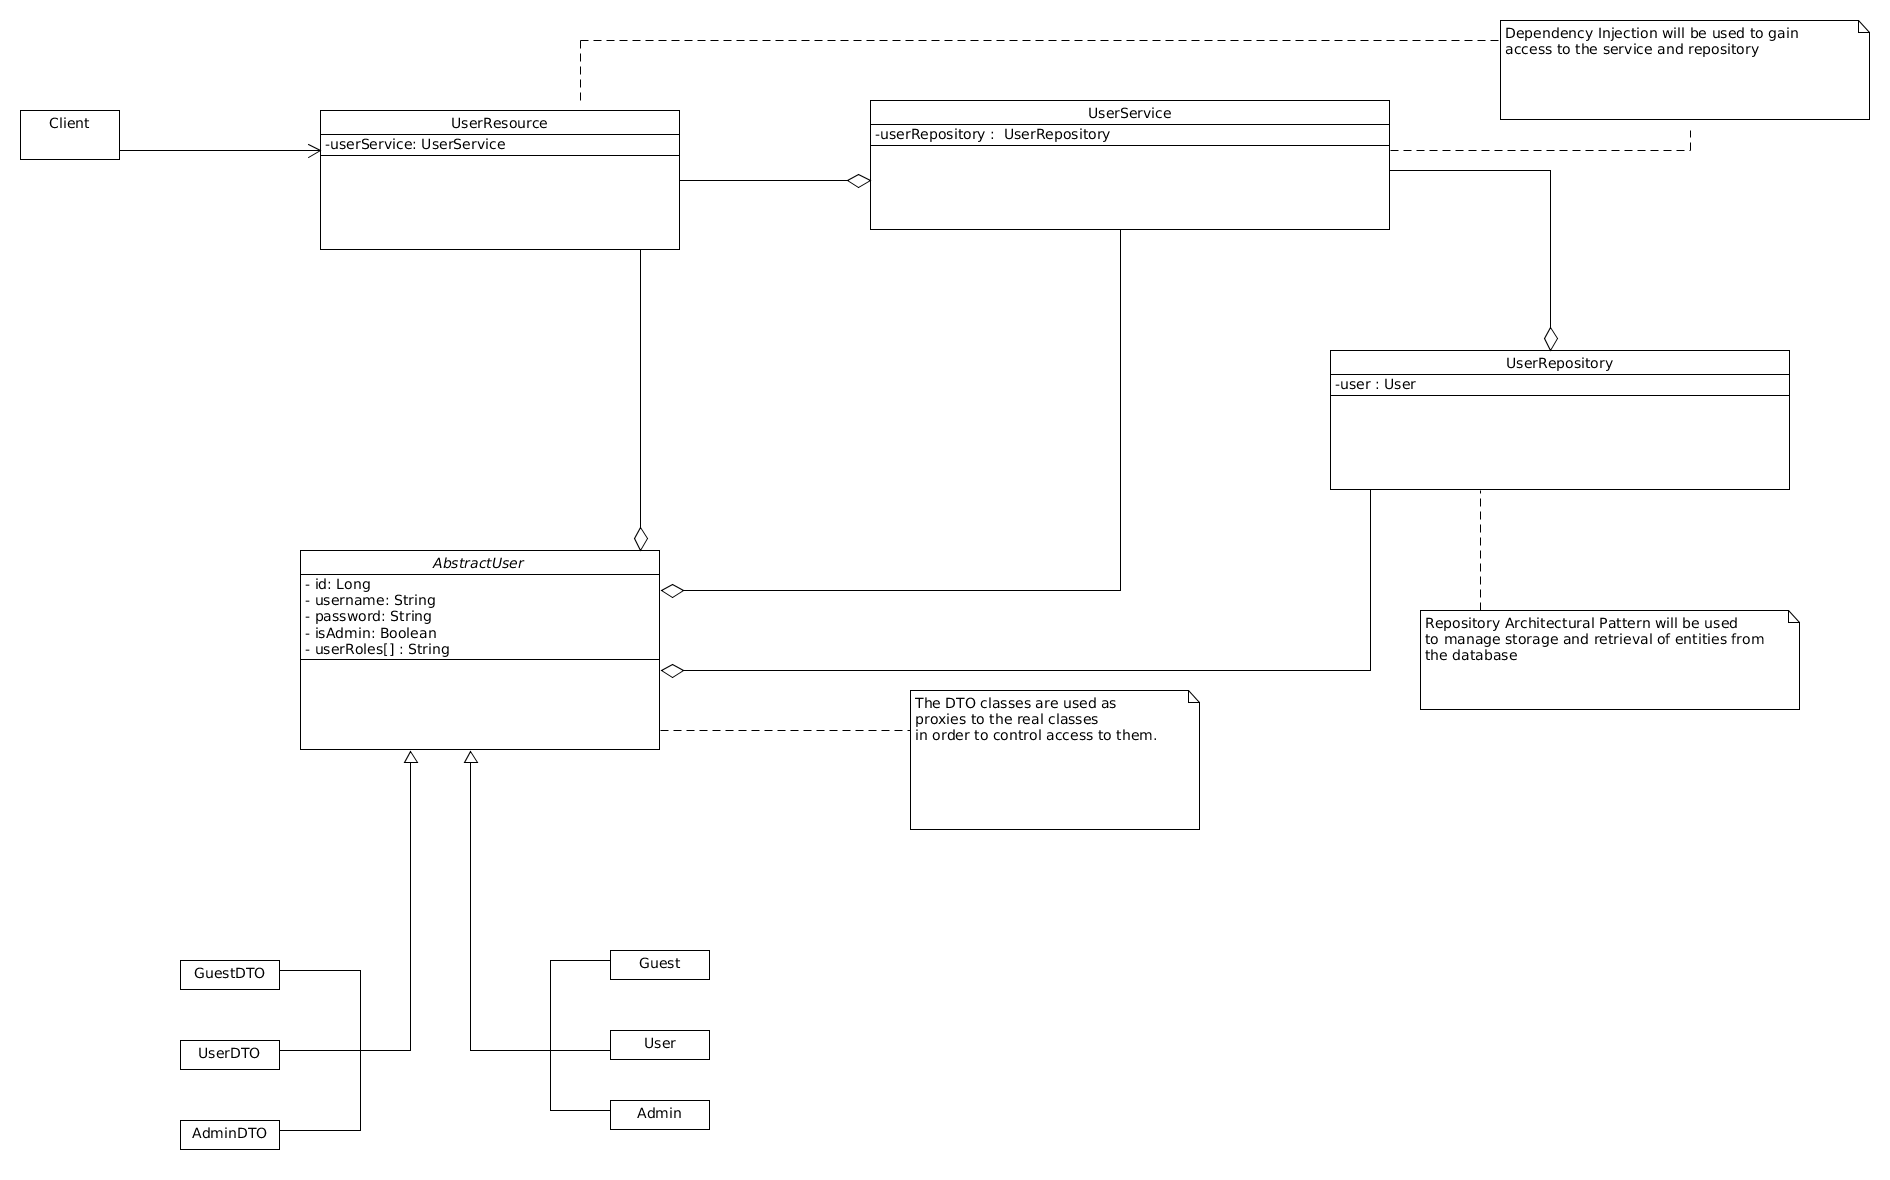
\includegraphics[width=0.7\textwidth]{User_Class_Diagrams.png}
   	\caption{Class Diagram for the User Module}
\end{figure}
\subsubsection {Explanation of Design Patterns in User Module}
\begin{itemize}
\item \underline{Proxy Pattern} The Proxy pattern has been used in the users module in order to control access to the user profiles within the backend application. By doing this we add a wrapper and delegation to protect the real component from complexity. 

\item The Data Transfer Objects (DTO's)  can have extra / less fields depending on what the client is or is not allowed to see in the user object. Typically the user object will have more fields than the DTO ( such as roles, hashes of passwords etc). 

\item \underline{Repository Pattern} The Repository Architectural Pattern will be used to manage database access. This pattern enables direct mapping of database objects / row entries to classes. It also delegates the responsibilty of managing the database to a single object. Listed below are a few advantages of using the Repository pattern:
	\begin{itemize}
		\item Enables one to maximize the amount of code that can be tested and isolate the data layer to support unit testing. 
		\item Enable one to access the data source from many locations by using dependency injection as well as apply centrally managed, consistent access rules and logic.
		\item Improve maintainability and readability of code by separating business logic from data access logic.  
	\end{itemize} 
\end{itemize}
\subsubsection {Activity Diagram for the User Login Use Case}
 	\begin{figure}[H]
   	\centering
   	\includegraphics[width=0.7\textwidth]{login_activity_diagram.png}
   	\caption{Activity Diagram for the Users Module, Login Use Case}
	\end{figure}
	
	This activity diagram serves to illustrate the flow or actions that will be performed by the system when a user logs onto the system. The getUser() service in the system will be used to retrieve user information to display on the web front-end once a user has been successfully validated and logged in. 
\subsubsection {Sequence Diagram for the User Register Use Case}
 	\begin{figure}[H]
   	\centering
   	\includegraphics[width=0.7\textwidth]{register_sequence_diagram.png}
   	\caption{Sequence Diagram for the Users Module, Register Use Case}
	\end{figure}
	
	The register user use case is described as follows: 
	\begin{itemize}
		\item The user clicks on register on the web browser in order to register their filled in information. 
		\item The web client then creates a REST API call with the POST method to create the user. This request is captured from a REST endpoint in the backend of the application.
		\item When the request is captured in the backend, it is mapped to the userDTO object so that the system can parse the fields in the request body elegantly. 
		\item The userResource then makes use of \textbf{dependency injection} by injecting the UserService into the class. The resource then invokes the createUser() method of the userService. This method will typically expect a UserDTO object to be passed as parameter.
		\item The user service will then instantiate a User object and map the required information from the userDTO to the user object. 
		\item The userRepository service is used in the UserService class via dependecy injection as well. The save() method is invoked which will save the user entry into the database. 
		\item After saving the user details, the repository returns a User object back to the user service. The user service then creates a results userDTO object to return. 
		\item The user object that has been returned from the repository is then mapped to the userDTO that will be returned to the userResource. 
		\item The userResource receives the responseDTO and sends it as a response to the client. This object will be in JSON format. 
	\end{itemize}

\subsection {Navigation}

\begin{figure}[H]
   	\centering
   	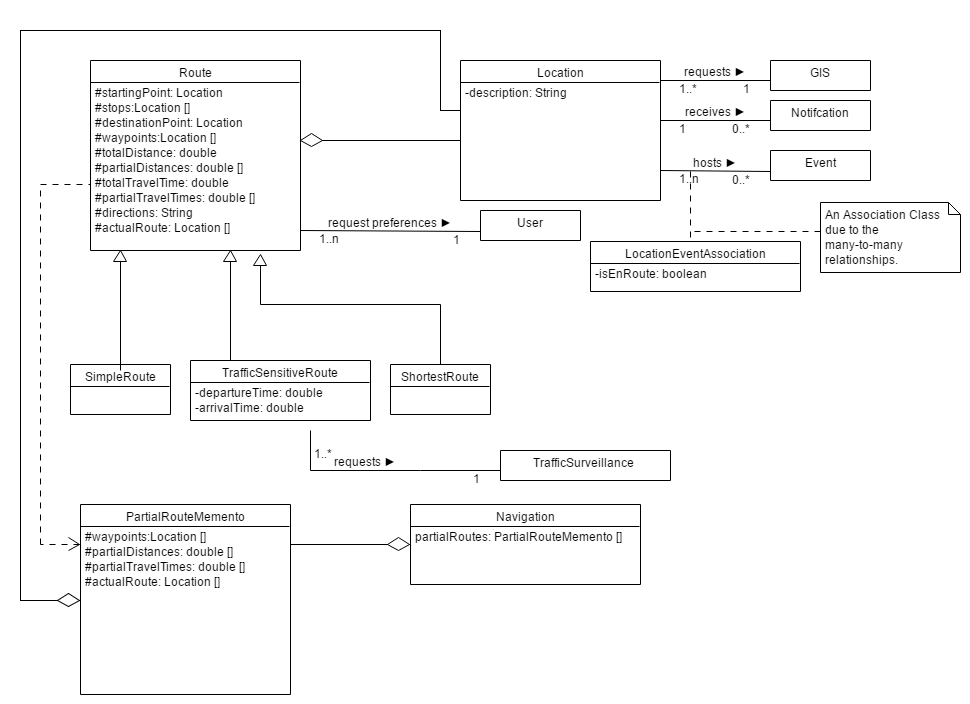
\includegraphics[width=0.7\textwidth]{Navigation-Module-Class-Diagram.png}
   	\caption{Class Diagram for the Navigations Module}
\end{figure}

\subsubsection {Explanation of Design Patterns in Navigation Module}
\begin{itemize}

\item \underline{Memento Pattern} - The Memento Pattern has been used in the navigation module in order to capture the internal state of a "route" object while the route is being calculated.
\item The internal state of the route that we would like to capture is the respective arrays for waypoints, partial distances, partial times and actual distances in the route. 
\item While routing, connection can be lost or the user may diverge from the specified paths during which the system will have to save the internal state so that it can return to this state at a later stage.
\item The role-back function in this case would be the re-route function.
\item The originator in the module is the Route class.
\item The caretaker is the Navigation class.
\item The memento is the PartialRouteMemento class.

\item \underline{Strategy Pattern} - The Strategy Pattern has been used in the navigation module in order to define a family of routing algorithms and make them interchangeable.
\item The users of the system will specify by clicking on different icons, the type of routing they want.
\item The abstraction class would be the Route class which is the interface to the user and is very generic with fundamental functionality.
\item The implementation classes would be the SimpleRoute, ShortestRoute and TrafficSenstiveRoute classes that will override the functionality of the superclass with algorithms for their respective needs.

\end{itemize}

\begin{figure}[H]
   	\centering
   	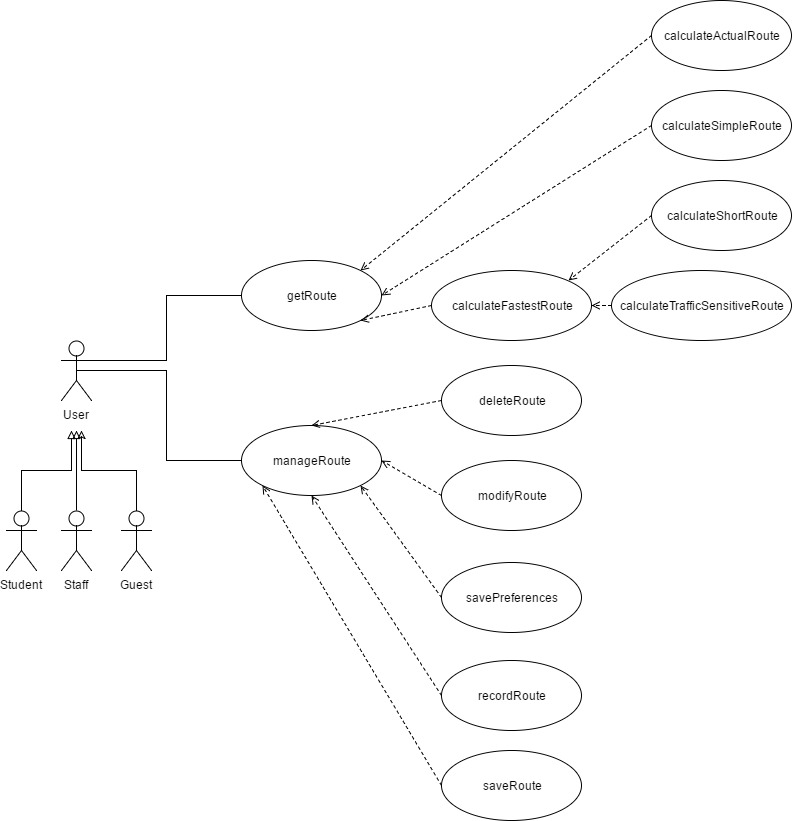
\includegraphics[width=0.7\textwidth]{Navigation-Module-Use-Case.jpg}
   	\caption{Use Case Diagram for the Navigations Module}
\end{figure}

\subsubsection {External Interface Requirements}
The navigation system communicates to three main entities; the network, the user and the user’s device. There needs to be an interface between each one of these entities to allow communication.

\begin{itemize}
\item \underline{User interface:} 
The user interacts with the navigation system via the GUI. This GUI needs to be flexible enough to function on devices of various sizes and operating systems. The interface must allow the user to have some method of control over the navigation system like choosing destinations, waypoints, routes and changes in these routes. 

\item The navigation system should also communicate to the user by showing information on the screen and through audio. This information includes messages on the screen, the map, locations on the map and the possible routes on the map.

\item Other aspects of the user interface like font, icons and the more visual aspects will be decided upon when the GUI is created.

\item \underline{Device Interface:}
\item In order to allow communication between the device and the navigation system, an interface needs to be created. The navigation system needs access and information from the device in order to function. This includes access to its hardware like the screen, device memory, connection to Wi-Fi or the internet, the location system and information like the device identity. 

\item The navigation system will be installed on the device along with the application. Being on the device itself will give it the needed access, if permission was granted. 

\item \underline{Network Interface:}
\item The navigation system functions best with communication between it and the network. This connection is established through the device’s connection. The connection can be to a WI-FI network or the mobile data network. 

\item The interface needs to facilitate exchange of information like location, identity, traffic, route information and aspects that might influence how navigation will take place. These aspects can be events, personal preference or personal information like disabilities. 

\end{itemize}

\subsubsection {Design Constraints}
The navigation system is constrained by the device hardware, access to information and the network connection.

\begin{itemize}
\item The hardware has direct influence on the efficiency of the navigation system. Poor hardware will lead to the navigation system working too slowly. Since this application must function effectively on various types of hardware, it is constrained to popular, rather simple hardware that is common amongst students. For example, it has to function fluently on both the newest smartphones and the older versions like the Samsung Galaxy S3.

\item The navigation system’s efficiency is also constrained to its ability to connect and communicate to the WI-FI and mobile networks. Since it uses the internet to get a constant flow of data that is used to navigate. This information included current location, heat-maps and events. This information is used to determine the best routes.

\item A constraint to the navigation system accuracy is the accuracy of the location system (GIS). The navigation system uses the location system to find its own location as well as locations of other buildings and areas on the map. If the location is inaccurate, the navigation system might give incorrect routes. 

\end{itemize}

\subsubsection {Software System Attributes}
\begin{itemize}
\item \underline{Reliability:} 
\item This navigation system must be able to function in a WI-FI or internet covered environment as well as a non-covered area up to some extent. Every location on campus must be available on the application. 

\item \underline{Security:}
\item This navigation system should function without releasing any user information to other devices. This navigation system should not access or be used to access any unneeded information on the user’s device. 
The user should also have a method of control over the information disseminated to the navigation system.

\item \underline{Availability:}
\item The navigation system must be part of the original application. It should be activated when the user choose a route to take instead of constantly calculating routes or finding locations. 

\item \underline{Interoperability:}
\item The navigation system must function on Android, iOS and in a web-browser.

\item \underline{Accuracy:}
\item The navigation system must be accurate up to 3m to function indoors but can be less accurate outdoors. 
\end{itemize}

=======
\subsection {Notifications}



\subsubsection{External Interface Requirements}
\mbox{}\\
The notification system consists of three parts: Software, Hardware and User interface. In order for the notification system to function properly, all three should be able to communicate and work together to perform the required tasks. 


\paragraph{Software Interface}
\mbox{}\\
The mobile application will connect to the database in order to obtain the users’ information. One such example includes obtaining information regarding the individuals selected notification medium. The mobile application will also connect to the server in order to update information regarding the users email address and mobile number.

\mbox{}\\
The server will be connected to the notification plugins, which include email and SMS plugins, as well as the application itself in times when notifications are displayed as a pop-up on the users’ mobile device.



\paragraph{Hardware Interface}

\mbox{}\\
The user will interact with the mobile device screen in order to set their notification medium preference that is sent and stored on the server. 

\mbox{}\\
When there is a notification, the server will then send data packets to the mobile application by making use of sockets. This will cause the mobile device to display the message as well as vibrate or make a sound. 

\mbox{}\\
The user will once again interact with the screen on their mobile device in order to view the notification.

\paragraph{User Interface}
\mbox{}\\
The user will initially interact with the notifications module through the application’s GUI where they will request to be notified about a certain event as well as provide their chosen notification medium. 

\mbox{}\\
If the chosen notifications medium is email, the user will receive a generic email with the given notification. The email will provide a description of the notification in its title. If required, the email will provide a link to the relevant website for more information concerning the notification. If the user selected to receive notifications via SMS, a message describing the notification will be sent to each user. Once again, a link will be provided in the SMS for more information concerning the notification as required. If the user decided to receive notifications through the application, a pop-up will appear on the applications’ GUI when there is a notification. 

\subsubsection{Performance Requirements}
\mbox{}\\
The system should be able to send out a large number of notifications without any delay (within 5 seconds).\\
Multiple administrators should be able to add new notifications without failure.



\subsubsection{Design Constraints}

The server should be able to hold an ever-increasing number of users mobile numbers as well as email addresses without failure.  

The user will require both a mobile number or email address and a mobile device with the application installed.

\subsubsection{Software System Attributes}
\begin{enumerate}

\item[•]Flexibility: The notifications system should be implemented in such a way that it will allow for the addition of new notification means.

\item[•]Maintainability: The notifications module should be implemented in such a way that future development is allowed. To achieve this, developers should write understandable and well documented code.
 
\item[•]Scalability: The database should be able to hold a large amount of users contact information as well as be able to notify a large amount of users at the same time.

\item[•]Reliability: The notifications module should ensure that all the users receive their required notifications.

\item[•]Security: The contact information of the users should be kept secure in order to ensure that third parties do not have access to it. This means that only authorised individuals should be able to access the contact information of the users.

\item[•]Auditability: The system should keep track of the sent and requested notifications.

\item[•]Testability: The notification service should be tested as a whole as well as in isolation regularly to ensure that the notification system still works optimally.

\item[•]Usability: The user should be able to clearly see that the pop-up is a notification.

\item[•]Integrability: The system should allow for future expansions.
\item[•]Scalability: The system will initially be implemented to navigate around the UP campus, but it might be necessary in the future to expand it to manage other facilities such as campuses and mall, therefore it should be scalable to such a user per campus or facility.
\item[•]Usability: Users must be able to login, navigate to different locations. Utilize additional features provided by the application and logout without hassle. The interface should not be cluttered and should not contain redundant information. As management of information on the system is critical, accessing said information should be as simple as possible.
\item[•]Reliability: It is imperative that the system not experience unnecessary downtime (period of in-operation of the system), thus preventing users from navigating on the maps to specified destinations, or altering information on the system. Additionally there should not be frequent errors within normal operating parameters of the system. Thus simple logins (sessions), alterations on the database, from either users or admin, should not cause errors which affect the system as a whole.

\end{enumerate}



\subsubsection{UML Diagrams}
\paragraph{Class Diagram}
\begin{center}
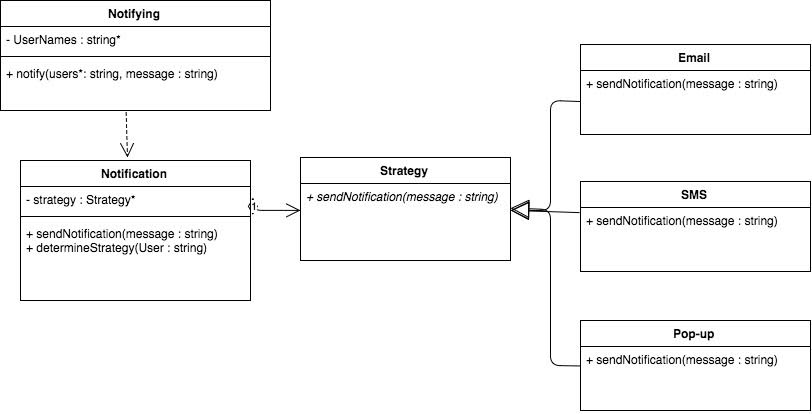
\includegraphics[width=10cm]{ClassDiagram.png}\\
\end{center}
\paragraph{Activity Diagram}
\begin{center}
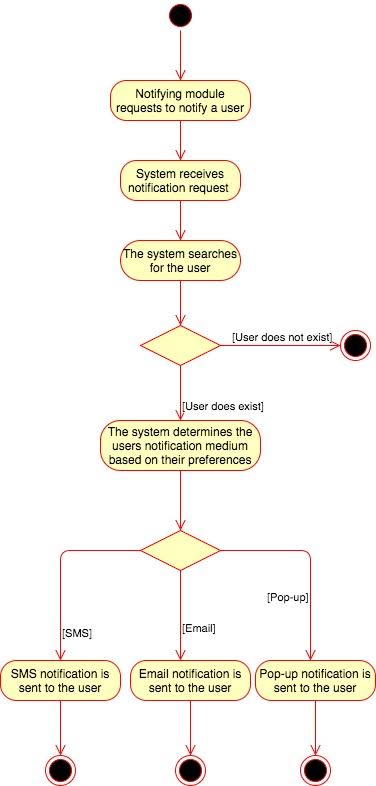
\includegraphics[height=10cm,width=5cm]{ActivityDiagram.png}\\ 
\end{center}
\paragraph{State Diagram}
\begin{center}
\includegraphics[height=10cm,width=5cm]{Notification-StateDiagram.png}\\ 
\end{center}
\paragraph{Use Case Diagram}
\begin{center}
\includegraphics[height=10cm,width=5cm]{Notification-UseCaseDiagram.png}\\ 
\end{center}






\subsubsection{Technology Choices}
Tuks email server will be used to notify the users.
Wi-Fi routers can be used to send the pop-up notifications to the application.
A SMS service can be used to notify the users.
\subsubsection{Explanation of Design Patterns in Notifications Module}
The strategy design pattern was used in the notifications module as it will allow for different mediums of communication to be used interchangeably.

The Context participant will be implemented with the Notification class. This class will be responsible for selecting which strategy will be used to notify the individual.

The Strategy in the design pattern will be implemented using the Strategy class. The responsibility of this class will be to call the required notification algorithm.

The Concrete Strategies will include the Email, SMS and Pop-up classes. These classes will responsible for implementing the different algorithms required for notifying the user based on their selected medium.


\subsection {Point of Interest}



\section{Technology Choices}



\section{References}

Kung, D.C. (2013) Object-oriented software engineering: An agile unified methodology. New York: McGraw Hill Higher Education.




\end{document}

